\pagestyle{plain}

\subsection{Exact structures}
\label{ss:genonexactstructure}

Let $\mathscr{A}$ be an abelian category.
%\benj{Dire quelques mots pour introduire des notations pour les suites exactes courtes ?}\Sunny{Ici, je trouve le tout très clair, je ne sais pas ce que tu avais en tête?} \benj{Je pense à amener quelques généralités : Qu'est-ce qu'une suite exacte ? Donner une notation propre aux suites exactes pour distinguer du Ext1 ? etc...} 
Recall that two short exact sequences in $\mathscr{A}$ \[\begin{tikzcd}
	\xi : & 0 & D & E & F &  0 \\
    \varsigma: & 0 & X & Y & Z &  0
	\arrow[from=1-2, to=1-3]
	\arrow["f",tail, from=1-3, to=1-4]
	\arrow["g",two heads,from=1-4, to=1-5]
	\arrow[from=1-5, to=1-6]
	\arrow[from=2-2, to=2-3]
	\arrow["i",tail, from=2-3, to=2-4]
	\arrow["j",two heads,from=2-4, to=2-5]
	\arrow[from=2-5, to=2-6]
\end{tikzcd} \] are said to be {\em isomorphic} whenever there exists a triplet of isomorphisms \[\left(\begin{tikzcd}
	D & X
	\arrow[Plum,"\phi",from=1-1, to=1-2]
\end{tikzcd}, \begin{tikzcd}
	E & Y
	\arrow[Plum,"\psi",from=1-1, to=1-2]
\end{tikzcd}, \begin{tikzcd}
	F & Z
	\arrow[Plum,"\mu",from=1-1, to=1-2]
\end{tikzcd} \right)\] such that every square in the following diagram commutes.
\[\begin{tikzcd}
	\xi : & 0 & D & E & F &  0 \\
    \varsigma: & 0 & X & Y & Z &  0
	\arrow[from=1-2, to=1-3]
	\arrow["f",tail, from=1-3, to=1-4]
        \arrow[Plum,"\phi",from=1-3, to=2-3]
	\arrow["g",two heads,from=1-4, to=1-5]
        \arrow[Plum,"\psi",from=1-4, to=2-4]
	\arrow[from=1-5, to=1-6]
        \arrow[Plum,"\mu",from=1-5, to=2-5]
	\arrow[from=2-2, to=2-3]
	\arrow["i",tail, from=2-3, to=2-4]
	\arrow["j",two heads,from=2-4, to=2-5]
	\arrow[from=2-5, to=2-6]
\end{tikzcd} \] 
From now on, by abusing notations, we identify a short exact sequence with its isomorphism class of short exact sequences. Fix a subcollection $\mathcal{E}$ of short exact sequences in $\mathscr{A}$. A short exact sequence \[\begin{tikzcd}
	\xi: & 0 & A & E & B &  0
	\arrow[from=1-2, to=1-3]
	\arrow["f",tail, from=1-3, to=1-4]
	\arrow["g",two heads,from=1-4, to=1-5]
	\arrow[from=1-5, to=1-6]
\end{tikzcd} \] is said to be \new{$\mathcal{E}$-exact} (or \new{$\mathcal{E}$-admissible}) if $\xi \in \mathcal{E}$. In such a case, we say that the map $f$ is said to be an \emph{$\mathcal{E}$-monomorphism}, and the map $g$ is said to be an \emph{$\mathcal{E}$-epimorphism}. Considering the short exact sequences up to isomorphism, the definitions of $\mathcal{E}$-exact sequences, $\mathcal{E}$-monomorphisms, and short $\mathcal{E}$-epimorphisms are interdependent, uniquely determining each other within this framework.

Quillen’s original formulation of exact structures thus encapsulates these relationships, providing a robust foundation for applying homological constructs in settings that deviate from traditional abelian categories. The Quillen definition can be rephrased as follows.

\begin{definition}\label{def:exact}
A collection $\mathcal{E}$ of short exact sequence in $\mathscr{A}$ is an \new{exact structure} on $\mathscr{A}$ whenever $\mathcal{E}$ satisfies the following axioms:
\begin{enumerate}[label=$(\mathsf{ES} \arabic*)$,itemsep=1mm]
    \item \label{ES1} All the split short exact sequences are in $\mathcal{E}$;
  
    \item \label{ES2} The collection of $\mathcal{E}$-monomorphisms and the one of $\mathcal{E}$-epimorphisms are both closed under compositions;
    
    \item\label{ES3} $\mathcal{E}$ is closed under the pushouts along any morphism: that is, any short exact sequence \[\begin{tikzcd}
	0 & X & Y & Z & 0 \\ 0 & D & PO & Z & 0 ,
	\arrow[from=1-1, to=1-2]
	\arrow["f",tail, from=1-2, to=1-3]
	\arrow[two heads,from=1-3, to=1-4]
	\arrow[from=1-4, to=1-5]
    \arrow[from=2-1, to=2-2]
	\arrow[tail, from=2-2, to=2-3]
	\arrow[two heads,from=2-3, to=2-4]
	\arrow[from=2-4, to=2-5]
    \arrow["h",from=1-2, to=2-2]
	\arrow[from=1-3, to=2-3]
    \arrow[equal,from=1-4, to=2-4]
 \end{tikzcd} \] where $f$ is an $\mathcal{E}$-monomorphism gives a short exact sequence is in $\mathcal{E}$ whenever taking the pushout along any morphism $h$;
    
\item \label{ES4} $\mathcal{E}$ is closed under the pullbacks along any morphism: that is, any short exact sequence \[\begin{tikzcd}
	0 & X & Y & Z & 0 \\ 0 & X & PB & F & 0 ,
	\arrow[from=1-1, to=1-2]
	\arrow[tail, from=1-2, to=1-3]
	\arrow["g",two heads,from=1-3, to=1-4]
	\arrow[from=1-4, to=1-5]
    \arrow[from=2-1, to=2-2]
	\arrow[tail, from=2-2, to=2-3]
	\arrow[two heads,from=2-3, to=2-4]
	\arrow[from=2-4, to=2-5]
    \arrow[equal,from=1-2, to=2-2]
	\arrow[from=2-3, to=1-3]
    \arrow["h",from=2-4, to=1-4]
 \end{tikzcd} \]where $g$ is an $\mathcal{E}$-epimorphism gives a short exact sequence in $\mathcal{E}$ whenever taking the pullback along any morphism $h$.
\end{enumerate}
If $\mathcal{E}$ is an exact structure on $\mathscr{A}$, then we refer to the pair $(\mathscr{A},\mathcal{E})$ as an \new{exact category}. We also refer to the exact structure containing all short exact sequences as $\mathcal{E}_{\max}$, and the one containing uniquely the split short exact sequences as $\mathcal{E}_{\min}$. We denote the subbifunctor of $\Ext^1_\mathscr{A}(-,-)$ as $\mathcal{E}(-,-)$, which selects only the extensions in $\mathcal{E}$. 
\end{definition}

\begin{definition}\label{def:Eprojectivesinjectives}
Let $(\mathscr{A}, \mathcal{E})$ be an exact category.
\begin{enumerate}[label=$\bullet$,itemsep=1mm]
    \item An object $P$ in $\mathscr{C}$ is \new{$\mathcal{E}$-projective} if for every $\mathcal{E}$-epimorphism $g: Y \to Z$, the map $g_* = \Hom_\mathscr{A}(P,g)$ is an epimorphism across all $Y, Z$ in $\mathscr{C}$. Equivalently, $P$ is $\mathcal{E}$-projective if the functor $\Hom_\mathscr{A}(P,-)$ preserves the $\mathcal{E}$-exactness of sequences. We write $\proj_\mathcal{E}(\mathscr{A})$ for the collection of $\mathcal{E}$-projective objects in $\mathscr{A}$. We observe that $\proj_{\mathcal{E}_{\max}}(\mathscr{A}) = \proj(\mathscr{A})$.
    \item An object $I$ in $\mathscr{C}$ is \new{$\mathcal{E}$-injective} if for every $\mathcal{E}$-monomorphism $f: X \to Y$, the map $f^* = \Hom_\mathscr{C}(f,I)$ is an epimorphism across all $X, Y$ in $\mathscr{C}$. Equivalently, $I$ is $\mathcal{E}$-injective if the functor $\Hom_\mathscr{C}(-,I)$ preserves the $\mathcal{E}$-exactness of sequences. We write $\inj_{\mathcal{E}}(\mathscr{A})$ for the collection of $\mathcal{E}$-injective objects in $\mathscr{A}$. We observe that $\inj_{\mathcal{E}_{\max}}(\mathscr{A}) = \inj(\mathscr{A})$.
\end{enumerate}
\end{definition}

We recall and restate some beneficial results on diagrams where the exact structure $\mathcal{E}$ intervenes, based on the work of T. Bühler \cite{B10}.

\begin{lemma}[$3 \times 3$-lemma] \label{lem:3x3}
Let $(\mathscr{A}, \mathcal{E})$ be an exact category. Consider the following commutative diagram.
\[\begin{tikzcd}
         & 0 & 0 & 0 &  \\
	& A & B  & C &   \\
      & A' & B' & C' &  \\
       & A'' & B'' & C'' &  \\
       & 0 & 0 & 0 & 
	%\arrow[from=2-1, to=2-2]
	\arrow[from=2-2, to=2-3]
	\arrow[from=2-3, to=2-4]
	%\arrow[from=2-4, to=2-5]
        %\arrow[from=3-1, to=3-2]
	\arrow["f",from=3-2, to=3-3]
	\arrow["g",from=3-3, to=3-4]
	%\arrow[from=3-4, to=3-5]
        %\arrow[from=4-1, to=4-2]
	\arrow[from=4-2, to=4-3]
	\arrow[from=4-3, to=4-4]
	%\arrow[from=4-4, to=4-5]
        \arrow[from=4-2, to=5-2]
	\arrow[two heads, from=3-2, to=4-2]
	\arrow[tail,from=2-2, to=3-2]
	\arrow[from=1-2, to=2-2]
        \arrow[from=4-3, to=5-3]
	\arrow[two heads, from=3-3, to=4-3]
	\arrow[tail,from=2-3, to=3-3]
	\arrow[from=1-3, to=2-3]
        \arrow[from=4-4, to=5-4]
	\arrow[two heads, from=3-4, to=4-4]
	\arrow[two heads,from=2-4, to=3-4]
	\arrow[from=1-4, to=2-4]
\end{tikzcd} \]
Assume that:
\begin{enumerate}[label=$\bullet$, itemsep=1mm]
    \item all the short sequences given by the columns are $\mathcal{E}$-exact; and,
    \item one of the following assertions holds:
    \begin{enumerate}[label=$\bullet$,itemsep=1mm]
        \item two out of the three rows, including the middle one, give short $\mathcal{E}$-exact sequences; or,
        \item the short sequences given by the top and the bottom rows are $\mathcal{E}$-exact, and $gf = 0$.
    \end{enumerate}
\end{enumerate}
Then the short sequence given by the remaining row is $\mathcal{E}$-exact.
\end{lemma}

\begin{remark} \label{rem:dual3x3}
    We can exchange the role of the rows and the columns to get a dual result applied on the columns of such a diagram.
\end{remark}

\begin{lemma}[Obscure axiom] \label{lem:obscure}
Let $(\mathscr{A}, \mathcal{E})$ be an exact category. Let $X,Y \in \mathscr{A}$ and $i : X \longrightarrow Y$. If there exist $Z \in \mathscr{A}$, and $j : Y \longrightarrow Z$ such that $j \circ i$ is an $\mathcal{E}$-monomorphism, then $i$ is an $\mathcal{E}$-monomorphism. Dually, it holds for $\mathcal{E}$-epimorphisms.
\end{lemma}

\begin{remark} \label{rem:obscure}
    This lemma was originally stated as an axiom from D. Quillen's definition of an exact category \cite{Q73}. At that time, N. Yoneda proved in his thesis \cite{Y61} that this axiom is a consequence of the other axioms. Later on, B. Keller \cite{K90} rediscovered this redundancy. The name ``obscure axiom" was given by R. W. Thomason and T. Trobaugh \cite{TT07}
\end{remark}

\subsection{Gen-Sub operators}
\label{ss:GenSuboperators}

Fix $(\mathscr{A},\mathcal{E})$ an exact category. 

\begin{definition} \label{def:Eadpted}
    A full subcategory $\mathscr{D} \subseteq \mathscr{A}$ is \new{$\mathcal{E}$-adapted} if for any pair $(X,Y)$ of objects in $\mathscr{C}$, we have $\Ext^1(X,Y) \subseteq \mathcal{E}$
\end{definition}
\begin{ex} $ $
\begin{enumerate}[label=$\bullet$, itemsep=1mm]
    \item Any full subcategory of $\mathscr{A}$ is $\mathcal{E}_{\max}$-adapted.
    \item A full subcategory $\mathscr{C} \subseteq \mathscr{A}$ is $\mathcal{E}_{\min}$-adapted only if for any $(X,Y) \in \mathscr{C}^2$, we have $\Ext_\mathscr{A}^1 (X,Y) = 0$.
\end{enumerate}

\end{ex}
This section introduces a closure operator on subcategories of $\mathscr{A}$. More precisely, given a subcategory $\mathscr{C}$, we will construct the smallest subcategory $\mathscr{D} \supseteq \mathscr{C}$ such that:
\begin{enumerate}[label=$\bullet$,itemsep=1mm]
    \item $\mathscr{D}$ is closed under cokernel of $\mathcal{E}$-monomorphisms; and,
    \item  $\mathscr{D}$ is closed under kernel of $\mathcal{E}$-epimorphisms.
\end{enumerate}

The \new{$\Gen_\mathcal{E}$-operator} on subcategories of $\mathscr{A}$ is defined as follows: given a subcategory $\mathscr{C} \subseteq \mathscr{A}$, we define $\Gen_\mathcal{E}(\mathscr{C})$ as the full subcategory, closed under sums and summands, of $\mathscr{A}$ containing the cokernel of any $\mathcal{E}$-monomorphism $f : X \longrightarrow Y$ such that $Y \in \mathscr{C}$. The \new{$\Sub_\mathcal{E}$-operator} on subcategories of $\mathscr{A}$ is defined analogously: given a subcategory $\mathscr{C} \subseteq \mathscr{A}$, we define $\Sub_\mathcal{E}(\mathscr{C})$ as the full subcategory, closed by sums and summands, of $\mathscr{A}$ containing the kernel of any $\mathcal{E}$-epimorphism $g : Y \longrightarrow X$  such that $Y \in \mathscr{C}$. Given an object $M \in \mathscr{C}$, by abusing of notation, we set $\Gen_\mathcal{E}(M) = \Gen_\mathcal{E}(\add(M))$ and $\Sub_\mathcal{E}(M) = \Sub_\mathcal{E}(\add(M))$.

Note that $\Gen_{\mathcal{E}_{\max}}(\mathscr{C}) = \Gen(\mathscr{C})$ and $\Sub_{\mathcal{E}_{\max}}(\mathscr{C}) = \Sub(\mathscr{C})$. As $\mathcal{E}$ is an exact structure on $\mathscr{A}$, then $\mathscr{C}$ is a subcategory of both $\Gen_\mathcal{E}(\mathscr{C})$ and $\Sub_\mathcal{E}(\mathscr{C})$. %\benj{Penses-tu qu'on puisse dire des choses sur l'intersection des deux ?}
%\Sunny{Si la catégorie $\mathscr{C}$ est partiellement tilting, l'intersection se trouve dans les compléments de $\mathscr{C}$, sinon ça peut-être n'importe quoi.}

Given a subcategory $\mathscr{C} \subseteq \mathscr{A}$, we define a sequence of subcategories $(\GS_{\mathcal{E}}^i(\mathscr{C}))_{i\in \mathbb{N}}$ as it follows:
\begin{enumerate}[label=$\bullet$, itemsep=1mm]
    \item we set $\GS_{\mathcal{E}}^0(\mathscr{C}) = \mathscr{C}$; and,
    \item for all $i \geqslant 1$, we define $\GS^{i}_{\mathcal{E}}(\mathscr{C})$ to be the full additive subcategory of $\mathscr{A}$ whose objects are given by both those in $\Gen_{\mathcal{E}}(\GS^{i-1}_{\mathcal{E}}(\mathscr{C}))$, and those in $\Sub_{\mathcal{E}}(\GS^{i-1}_{\mathcal{E}}(\mathscr{C}))$.
\end{enumerate}
By the previous remark, $(\GS_{\mathcal{E}}^i(\mathscr{C}))_{i\in \mathbb{N}}$ is an increasing sequence of additive subcategories of $\mathscr{A}$. Therefore, as $\mathscr{A}$ is abelian, this sequence of subcategories admits a colimit.

\begin{definition} \label{def:GSop}
    The \new{$\GS_\mathcal{E}$-operator} on subcategories of $\mathscr{A}$ is defined as follows: given a subcategory $\mathscr{C} \subseteq \mathscr{A}$, we define $\GS_{\mathcal{E}}(\mathscr{C})$ as the colimit of the sequence of subcategories $(\GS_\mathcal{E}^i(\mathscr{C}))_{i\in \mathbb{N}}$. As before, we set $\GS_\mathcal{E}(M) = \GS_\mathcal{E}(\add(M))$ by abuse of notations.
\end{definition}

Here are some apparent results coming directly from the definition.

\begin{lemma} \label{lem:proponGS}
Let $\mathscr{C} \subseteq \mathscr{A}$. The following assertions hold:
\begin{enumerate}[label=$(\alph*)$,itemsep=1mm]
    \item The category $\GS_\mathcal{E}(\mathscr{C})$ is the full additive subcategory of $\mathscr{A}$ whose objects are the ones appearing in $\GS^i(\mathscr{C})$ for some $i \in \mathbb{N}$.
    \item  The category $\GS_\mathcal{E}(\mathscr{C})$ is the smallest subcategory $\mathscr{A}$ containing $\mathscr{C}$, closed under taking $\mathcal{E}$-subobjects and  $\mathcal{E}$-quotients. \benj{$\mathcal{E}-$Thick or Serre?} \Sunny{$\mathcal{E}$-Serre est la terminologie la plus utilisée, mais il faut avoir ext-closed aussi}
\end{enumerate}
\end{lemma}

\pagebreak
\begin{ex} Let $Q$ be the following quiver of type $\mathbb{A}_7$ and $\mathscr{C} \subseteq \rep(Q)$ be the subcategory defined by the indecomposable objects in the blue rectangles. 
    
\leavevmode\\[-0.5ex]  % forces heading to appear before content


\centering
 


    \begin{tikzpicture}
    
				\begin{scope}[line width=.5mm,->, >= angle 60]
                    \node at (-1,0){$Q:$};
					\node (a) at (0,0){$1$};
					\node (b) at (1,0){$2$};
					\node (c) at (2,0){$3$};
					\node (d) at (3,0){$4$};
                    \node (e) at (4,0){$5$};
                    \node (f) at (5,0){$6$};
                    \node (g) at (6,0){$7$};
					\draw (a) -- (b);
					\draw (c) -- (b);
					\draw (c) -- (d);
                    \draw (d) -- (e);
                    \draw (f) -- (e);
                    \draw (f) -- (g);
				\end{scope}

				\begin{scope}[yshift=-3cm, xshift=-.5cm, line width=.3mm, ->, >= angle 60]
					\node at (3,2){Auslander-Reiten quiver with $\GS^{0}_{\mathcal{E}_\diamond}(\mathscr{C}) = \mathscr{C} =\add$ 
                    \tikz[baseline=-0.5ex] \node[rectangle, line width=0mm, fill=bleudefrance!10, draw, minimum width=1em, minimum height=1em] {};};
					\node (2) at (0,0){\scalebox{.7}{
							\begin{tikzpicture}[scale=0.2]
								\node at (0,0){$2$};
					\end{tikzpicture}}};
					\node (12) at (1,1){\scalebox{.7}{
							\begin{tikzpicture}[scale=0.2]
								\node at (0,0){$1$};
								\node at (1,-1){$2$};
					\end{tikzpicture}}};
					\node (2345) at (1,-1){\scalebox{.7}{
							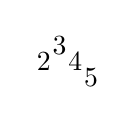
\begin{tikzpicture}[scale=0.2]
								\node at (-1,-1){$2$};
								\node at (0,0){$3$};
								\node at (1,-1){$4$};
                                \node at (2,-2){$5$};
					\end{tikzpicture}}};
					\node (45) at (0,-2){\scalebox{.7}{
							\begin{tikzpicture}[scale=0.2]
								\node at (0,0){$4$};
                                \node at (1,-1){$5$};
					\end{tikzpicture}}};
                    \node[rectangle,line width=0mm,fill=bleudefrance!10,draw] (5) at (-1,-3){\scalebox{.7}{
							\begin{tikzpicture}[scale=0.2]
                                \node at (0,0){$5$};
					\end{tikzpicture}}};
                    \node[rectangle,line width=0mm,fill=bleudefrance!10,draw] (567) at (0,-4){\scalebox{.7}{
							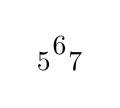
\begin{tikzpicture}[scale=0.2]
                                \node at (-1,-1){$5$};
								\node at (0,0){$6$};
								\node at (1,-1){$7$};  
					\end{tikzpicture}}};
                    \node (7) at (-1,-5){\scalebox{.7}{
							\begin{tikzpicture}[scale=0.2]
                                \node at (0,0){$7$};
					\end{tikzpicture}}};
                    \node (56)[rectangle,line width=0mm,fill=bleudefrance!10,draw] at (1,-5){\scalebox{.7}{
							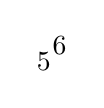
\begin{tikzpicture}[scale=0.2]
                                \node at (0,0){$6$};
                                \node at (-1,-1){$5$};
					\end{tikzpicture}}};
                     \node (4) at (3,-5){\scalebox{.7}{
							\begin{tikzpicture}[scale=0.2]
                                \node at (0,0){$4$};
					\end{tikzpicture}}};
                     \node[rectangle,line width=0mm,fill=bleudefrance!10,draw] (23) at (5,-5){\scalebox{.7}{
							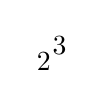
\begin{tikzpicture}[scale=0.2]
                                \node at (0,0){$3$};
                                \node at (-1,-1){$2$};
					\end{tikzpicture}}};
                    \node (1) at (7,-5){\scalebox{.7}{
							\begin{tikzpicture}[scale=0.2]
                                \node at (0,0){$1$};
					\end{tikzpicture}}};
                    \node (456) at (2,-4){\scalebox{.7}{
							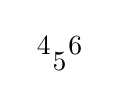
\begin{tikzpicture}[scale=0.2]
                                \node at (-1,1){$4$};
								\node at (0,0){$5$};
								\node at (1,1){$6$};  
					\end{tikzpicture}}};
                    \node (234) at (4,-4){\scalebox{.7}{
							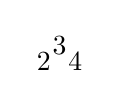
\begin{tikzpicture}[scale=0.2]
                                \node at (-1,-1){$2$};
								\node at (0,0){$3$};
								\node at (1,-1){$4$};  
					\end{tikzpicture}}};
                     \node[rectangle,line width=0mm,fill=bleudefrance!10,draw] (123) at (6,-4){\scalebox{.7}{
							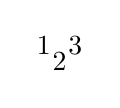
\begin{tikzpicture}[scale=0.2]
                                \node at (-1,1){$1$};
								\node at (0,0){$2$};
								\node at (1,1){$3$};  
					\end{tikzpicture}}};
                     \node (4567) at (1,-3){\scalebox{.7}{
							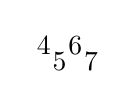
\begin{tikzpicture}[scale=0.2]
                                \node at (-2,0){$4$};
                                \node at (-1,-1){$5$};
								\node at (0,0){$6$};
								\node at (1,-1){$7$};  
					\end{tikzpicture}}};
                     \node (23456) at (3,-3){\scalebox{.7}{
							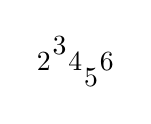
\begin{tikzpicture}[scale=0.2]
                               \node at (-1,-1){$2$};
								\node at (0,0){$3$};
								\node at (1,-1){$4$};
                                \node at (2,-2){$5$};
                                \node at (3,-1){$6$};
					\end{tikzpicture}}};
                     \node (1234) at (5,-3){\scalebox{.7}{
							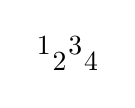
\begin{tikzpicture}[scale=0.2]
                                \node at (-2,0){$1$};
                                \node at (-1,-1){$2$};
								\node at (0,0){$3$};
								\node at (1,-1){$4$};

					\end{tikzpicture}}};
                     \node (3) at (7,-3){\scalebox{.7}{
							\begin{tikzpicture}[scale=0.2]
                                \node at (0,0){$3$};
					\end{tikzpicture}}};
					\node[rectangle,line width=0mm,fill=bleudefrance!10,draw] (12345) at (2,0){\scalebox{.7}{
							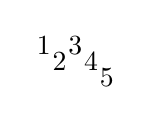
\begin{tikzpicture}[scale=0.2]
								\node at (-2,0){$1$};
								\node at (-1,-1){$2$};
								\node at (0,0){$3$};
								\node at (1,-1){$4$};
                                \node at (2,-2){$5$};
					\end{tikzpicture}}};
					\node (234567) at (2,-2){\scalebox{.7}{
							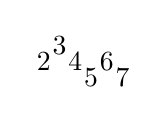
\begin{tikzpicture}[scale=0.2]
								 \node at (-1,-1){$2$};
								\node at (0,0){$3$};
								\node at (1,-1){$4$};
                                \node at (2,-2){$5$};
                                \node at (3,-1){$6$};
                                 \node at (4,-2){$7$};
					\end{tikzpicture}}};
                    \node (123456) at (4,-2){\scalebox{.7}{
							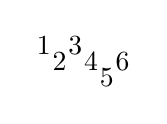
\begin{tikzpicture}[scale=0.2]
                                \node at (-2,0){$1$};
                                \node at (-1,-1){$2$};
								\node at (0,0){$3$};
								\node at (1,-1){$4$};
                                \node at (2,-2){$5$};
                                \node at (3,-1){$6$};
					\end{tikzpicture}}};
					\node (34) at (6,-2){\scalebox{.7}{
							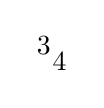
\begin{tikzpicture}[scale=0.2]
								\node at (0,0){$3$};
								\node at (1,-1){$4$};
					\end{tikzpicture}}};
					\node (1234567) at (3,-1){\scalebox{.7}{
							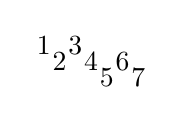
\begin{tikzpicture}[scale=0.2]
                                \node at (-2,0){$1$};
                                \node at (-1,-1){$2$};
								\node at (0,0){$3$};
								\node at (1,-1){$4$};
                                \node at (2,-2){$5$};
                                \node at (3,-1){$6$};
                                \node at (4,-2){$7$};
					\end{tikzpicture}}};
                    \node (3456) at (5,-1){\scalebox{.7}{
							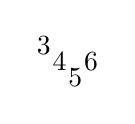
\begin{tikzpicture}[scale=0.2]
								\node at (3,-1){$6$};
								\node at (0,0){$3$};
								\node at (1,-1){$4$};
                                \node at (2,-2){$5$};
					\end{tikzpicture}}};
                    \node (34567) at (4,0){\scalebox{.7}{
							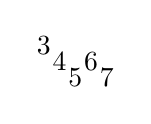
\begin{tikzpicture}[scale=0.2]
								\node at (0,0){$3$};
								\node at (1,-1){$4$};
                                \node at (2,-2){$5$};
                                \node at (3,-1){$6$};
                                 \node at (4,-2){$7$};
                    \end{tikzpicture}}};
                    \node (6) at (6,0){\scalebox{.7}{
							\begin{tikzpicture}[scale=0.2]
                                \node at (0,0){$6$};
                    \end{tikzpicture}}};
                    \node[rectangle,line width=0mm,fill=bleudefrance!10,draw] (345) at (3,1){\scalebox{.7}{
							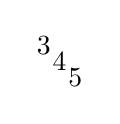
\begin{tikzpicture}[scale=0.2]
								\node at (0,0){$3$};
								\node at (1,-1){$4$};
                                \node at (2,-2){$5$};
                    \end{tikzpicture}}};
                    \node (67) at (5,1){\scalebox{.7}{
							\begin{tikzpicture}[scale=0.2]
								\node at (0,0){$6$};
								\node at (1,-1){$7$};
					\end{tikzpicture}}};
					\draw (2) -- (12);
					\draw (2) -- (2345);
					\draw (45) -- (2345);
					\draw (12) -- (12345);
					\draw (2345) -- (12345);
					\draw (2345) -- (234567);
                    \draw (12345) -- (345);
                    
                    
                    \draw (5) -- (45);
                    \draw (7) -- (567);
                    \draw (567) -- (4567);
                    \draw (4567) -- (234567);
                    \draw (234567) -- (1234567);
                    \draw (1234567) -- (34567);
                    \draw (34567) -- (67);
                    \draw (56) -- (456);
                    \draw (456) -- (23456);
                    \draw (23456) -- (123456);
                    \draw (123456) -- (3456);
                    \draw (3456) -- (6);
                    \draw (4) -- (234);
                    \draw (234) -- (1234);
                    \draw (1234) -- (34);
                    \draw (23) -- (123);
                    \draw (123) -- (3);
					
					\draw (5) -- (567);
                    \draw (567) -- (56);
                    \draw (45) -- (4567);
                    \draw (4567) -- (456);
                    \draw (456) -- (4);
                    \draw (234567) -- (23456);
                    \draw (23456) -- (234);
                    \draw (234) -- (23);
                    \draw (12345) -- (1234567);
                    \draw (1234567) -- (123456);
                    \draw (123456) -- (1234);
                    \draw (1234) -- (123);
                    \draw (123) -- (1);
                    \draw (345) -- (34567);
                    \draw (34567) -- (3456);
                    \draw (3456) -- (34);
                    \draw (34) -- (3);
                    \draw (67) -- (6);
                    
                    
                    
    

                    
                    
					
					
				
					
				\end{scope}
               
    \end{tikzpicture}
  
By taking all the short exact sequences in $\mathcal{E}_\diamond$ whose middle terms lie in $\mathscr{C}$, we define $\GS^{1}_{\mathcal{E}_\diamond}(\mathscr{C})$ by adding the end terms of these sequences to the subcategory $\mathscr{C}$.
    
    \vspace{1cm}

    
    \begin{tikzpicture}
        \begin{scope}[yshift=-3cm, xshift=-.5cm, line width=.3mm, ->, >= angle 60]
					\node at (3,2) {$\GS^{1}_{\mathcal{E}_\diamond}(\mathscr{C}) =\add$};\node at (4.5,2) [rectangle,line width=0mm,fill=bleudefrance!10,draw, minimum width=1em,minimum height=1em] {};
					\node (2) at (0,0){\scalebox{.7}{
							\begin{tikzpicture}[scale=0.2]
								\node at (0,0){$2$};
					\end{tikzpicture}}};
					\node (12) at (1,1){\scalebox{.7}{
							\begin{tikzpicture}[scale=0.2]
								\node at (0,0){$1$};
								\node at (1,-1){$2$};
					\end{tikzpicture}}};
					\node[rectangle,line width=0mm,fill=bleudefrance!10,draw] (2345) at (1,-1){\scalebox{.7}{
							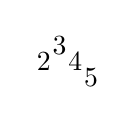
\begin{tikzpicture}[scale=0.2]
								\node at (-1,-1){$2$};
								\node at (0,0){$3$};
								\node at (1,-1){$4$};
                                \node at (2,-2){$5$};
					\end{tikzpicture}}};
					\node (45) at (0,-2){\scalebox{.7}{
							\begin{tikzpicture}[scale=0.2]
								\node at (0,0){$4$};
                                \node at (1,-1){$5$};
					\end{tikzpicture}}};
                    \node[rectangle,line width=0mm,fill=bleudefrance!10,draw] (5) at (-1,-3){\scalebox{.7}{
							\begin{tikzpicture}[scale=0.2]
                                \node at (0,0){$5$};
					\end{tikzpicture}}};
                    \node[rectangle,line width=0mm,fill=bleudefrance!10,draw] (567) at (0,-4){\scalebox{.7}{
							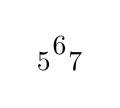
\begin{tikzpicture}[scale=0.2]
                                \node at (-1,-1){$5$};
								\node at (0,0){$6$};
								\node at (1,-1){$7$};  
					\end{tikzpicture}}};
                    \node (7) at (-1,-5){\scalebox{.7}{
							\begin{tikzpicture}[scale=0.2]
                                \node at (0,0){$7$};
					\end{tikzpicture}}};
                    \node (56)[rectangle,line width=0mm,fill=bleudefrance!10,draw] at (1,-5){\scalebox{.7}{
							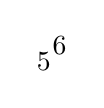
\begin{tikzpicture}[scale=0.2]
                                \node at (0,0){$6$};
                                \node at (-1,-1){$5$};
					\end{tikzpicture}}};
                     \node (4) at (3,-5){\scalebox{.7}{
							\begin{tikzpicture}[scale=0.2]
                                \node at (0,0){$4$};
					\end{tikzpicture}}};
                     \node[rectangle,line width=0mm,fill=bleudefrance!10,draw] (23) at (5,-5){\scalebox{.7}{
							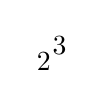
\begin{tikzpicture}[scale=0.2]
                                \node at (0,0){$3$};
                                \node at (-1,-1){$2$};
					\end{tikzpicture}}};
                    \node (1) at (7,-5){\scalebox{.7}{
							\begin{tikzpicture}[scale=0.2]
                                \node at (0,0){$1$};
					\end{tikzpicture}}};
                    \node (456) at (2,-4){\scalebox{.7}{
							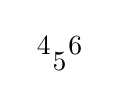
\begin{tikzpicture}[scale=0.2]
                                \node at (-1,1){$4$};
								\node at (0,0){$5$};
								\node at (1,1){$6$};  
					\end{tikzpicture}}};
                    \node (234) at (4,-4){\scalebox{.7}{
							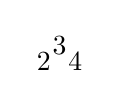
\begin{tikzpicture}[scale=0.2]
                                \node at (-1,-1){$2$};
								\node at (0,0){$3$};
								\node at (1,-1){$4$};  
					\end{tikzpicture}}};
                     \node[rectangle,line width=0mm,fill=bleudefrance!10,draw] (123) at (6,-4){\scalebox{.7}{
							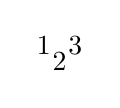
\begin{tikzpicture}[scale=0.2]
                                \node at (-1,1){$1$};
								\node at (0,0){$2$};
								\node at (1,1){$3$};  
					\end{tikzpicture}}};
                     \node (4567) at (1,-3){\scalebox{.7}{
							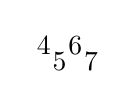
\begin{tikzpicture}[scale=0.2]
                                \node at (-2,0){$4$};
                                \node at (-1,-1){$5$};
								\node at (0,0){$6$};
								\node at (1,-1){$7$};  
					\end{tikzpicture}}};
                     \node (23456) at (3,-3){\scalebox{.7}{
							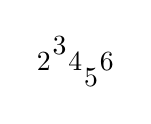
\begin{tikzpicture}[scale=0.2]
                               \node at (-1,-1){$2$};
								\node at (0,0){$3$};
								\node at (1,-1){$4$};
                                \node at (2,-2){$5$};
                                \node at (3,-1){$6$};
					\end{tikzpicture}}};
                     \node (1234) at (5,-3){\scalebox{.7}{
							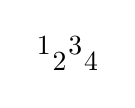
\begin{tikzpicture}[scale=0.2]
                                \node at (-2,0){$1$};
                                \node at (-1,-1){$2$};
								\node at (0,0){$3$};
								\node at (1,-1){$4$};

					\end{tikzpicture}}};
                     \node[rectangle,line width=0mm,fill=bleudefrance!10,draw] (3) at (7,-3){\scalebox{.7}{
							\begin{tikzpicture}[scale=0.2]
                                \node at (0,0){$3$};
					\end{tikzpicture}}};
					\node[rectangle,line width=0mm,fill=bleudefrance!10,draw] (12345) at (2,0){\scalebox{.7}{
							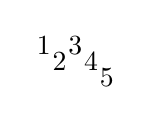
\begin{tikzpicture}[scale=0.2]
								\node at (-2,0){$1$};
								\node at (-1,-1){$2$};
								\node at (0,0){$3$};
								\node at (1,-1){$4$};
                                \node at (2,-2){$5$};
					\end{tikzpicture}}};
					\node (234567) at (2,-2){\scalebox{.7}{
							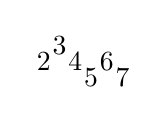
\begin{tikzpicture}[scale=0.2]
								 \node at (-1,-1){$2$};
								\node at (0,0){$3$};
								\node at (1,-1){$4$};
                                \node at (2,-2){$5$};
                                \node at (3,-1){$6$};
                                 \node at (4,-2){$7$};
					\end{tikzpicture}}};
                    \node[rectangle,line width=0mm,fill=bleudefrance!10,draw] (123456) at (4,-2){\scalebox{.7}{
							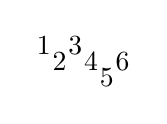
\begin{tikzpicture}[scale=0.2]
                                \node at (-2,0){$1$};
                                \node at (-1,-1){$2$};
								\node at (0,0){$3$};
								\node at (1,-1){$4$};
                                \node at (2,-2){$5$};
                                \node at (3,-1){$6$};
					\end{tikzpicture}}};
					\node (34) at (6,-2){\scalebox{.7}{
							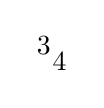
\begin{tikzpicture}[scale=0.2]
								\node at (0,0){$3$};
								\node at (1,-1){$4$};
					\end{tikzpicture}}};
					\node[rectangle,line width=0mm,fill=bleudefrance!10,draw] (1234567) at (3,-1){\scalebox{.7}{
							\begin{tikzpicture}[scale=0.2]
                                \node at (-2,0){$1$};
                                \node at (-1,-1){$2$};
								\node at (0,0){$3$};
								\node at (1,-1){$4$};
                                \node at (2,-2){$5$};
                                \node at (3,-1){$6$};
                                \node at (4,-2){$7$};
					\end{tikzpicture}}};
                    \node[rectangle,line width=0mm,fill=bleudefrance!10,draw] (3456) at (5,-1){\scalebox{.7}{
							\begin{tikzpicture}[scale=0.2]
								\node at (3,-1){$6$};
								\node at (0,0){$3$};
								\node at (1,-1){$4$};
                                \node at (2,-2){$5$};
					\end{tikzpicture}}};
                    \node[rectangle,line width=0mm,fill=bleudefrance!10,draw] (34567) at (4,0){\scalebox{.7}{
							\begin{tikzpicture}[scale=0.2]
								\node at (0,0){$3$};
								\node at (1,-1){$4$};
                                \node at (2,-2){$5$};
                                \node at (3,-1){$6$};
                                 \node at (4,-2){$7$};
                    \end{tikzpicture}}};
                    \node (6) at (6,0){\scalebox{.7}{
							\begin{tikzpicture}[scale=0.2]
                                \node at (0,0){$6$};
                    \end{tikzpicture}}};
                    \node[rectangle,line width=0mm,fill=bleudefrance!10,draw] (345) at (3,1){\scalebox{.7}{
							\begin{tikzpicture}[scale=0.2]
								\node at (0,0){$3$};
								\node at (1,-1){$4$};
                                \node at (2,-2){$5$};
                    \end{tikzpicture}}};
                    \node (67) at (5,1){\scalebox{.7}{
							\begin{tikzpicture}[scale=0.2]
								\node at (0,0){$6$};
								\node at (1,-1){$7$};
					\end{tikzpicture}}};
					\draw (2) -- (12);
					\draw (2) -- (2345);
					\draw (45) -- (2345);
					\draw (12) -- (12345);
					\draw (2345) -- (12345);
					\draw (2345) -- (234567);
                    \draw (12345) -- (345);
                    
                    
                    \draw (5) -- (45);
                    \draw (7) -- (567);
                    \draw (567) -- (4567);
                    \draw (4567) -- (234567);
                    \draw (234567) -- (1234567);
                    \draw (1234567) -- (34567);
                    \draw (34567) -- (67);
                    \draw (56) -- (456);
                    \draw (456) -- (23456);
                    \draw (23456) -- (123456);
                    \draw (123456) -- (3456);
                    \draw (3456) -- (6);
                    \draw (4) -- (234);
                    \draw (234) -- (1234);
                    \draw (1234) -- (34);
                    \draw (23) -- (123);
                    \draw (123) -- (3);
					
					\draw (5) -- (567);
                    \draw (567) -- (56);
                    \draw (45) -- (4567);
                    \draw (4567) -- (456);
                    \draw (456) -- (4);
                    \draw (234567) -- (23456);
                    \draw (23456) -- (234);
                    \draw (234) -- (23);
                    \draw (12345) -- (1234567);
                    \draw (1234567) -- (123456);
                    \draw (123456) -- (1234);
                    \draw (1234) -- (123);
                    \draw (123) -- (1);
                    \draw (345) -- (34567);
                    \draw (34567) -- (3456);
                    \draw (3456) -- (34);
                    \draw (34) -- (3);
                    \draw (67) -- (6);
                    
                    
                    
                    
                    
					
					
				
					
				\end{scope}
    \end{tikzpicture}

\centering
By taking all the short exact sequences in $\mathcal{E}_\diamond$ whose middle terms lie in  $\GS^{1}_{\mathcal{E}_\diamond}(\mathscr{C})$, we define $\GS^{2}_{\mathcal{E}_\diamond}(\mathscr{C})$ by adding the end terms of these sequences to the subcategory $\GS^{1}_{\mathcal{E}_\diamond}(\mathscr{C})$.
       \vspace{1cm}

    
    \begin{tikzpicture}
        \begin{scope}[yshift=-3cm, xshift=-.5cm, line width=.3mm, ->, >= angle 60]
					\node at (3,2){$\GS_{\mathcal{E}_\diamond}(\mathscr{C})=\GS^{2}_{\mathcal{E}_\diamond}(\mathscr{C}) =\add$};\node at (5.375,2) [rectangle,line width=0mm,fill=bleudefrance!10,draw, minimum width=1em,minimum height=1em] {};
					\node (2) at (0,0){\scalebox{.7}{
							\begin{tikzpicture}[scale=0.2]
								\node at (0,0){$2$};
					\end{tikzpicture}}};
					\node (12) at (1,1){\scalebox{.7}{
							\begin{tikzpicture}[scale=0.2]
								\node at (0,0){$1$};
								\node at (1,-1){$2$};
					\end{tikzpicture}}};
					\node[rectangle,line width=0mm,fill=bleudefrance!10,draw] (2345) at (1,-1){\scalebox{.7}{
							\begin{tikzpicture}[scale=0.2]
								\node at (-1,-1){$2$};
								\node at (0,0){$3$};
								\node at (1,-1){$4$};
                                \node at (2,-2){$5$};
					\end{tikzpicture}}};
					\node (45) at (0,-2){\scalebox{.7}{
							\begin{tikzpicture}[scale=0.2]
								\node at (0,0){$4$};
                                \node at (1,-1){$5$};
					\end{tikzpicture}}};
                    \node[rectangle,line width=0mm,fill=bleudefrance!10,draw] (5) at (-1,-3){\scalebox{.7}{
							\begin{tikzpicture}[scale=0.2]
                                \node at (0,0){$5$};
					\end{tikzpicture}}};
                    \node[rectangle,line width=0mm,fill=bleudefrance!10,draw] (567) at (0,-4){\scalebox{.7}{
							\begin{tikzpicture}[scale=0.2]
                                \node at (-1,-1){$5$};
								\node at (0,0){$6$};
								\node at (1,-1){$7$};  
					\end{tikzpicture}}};
                    \node (7) at (-1,-5){\scalebox{.7}{
							\begin{tikzpicture}[scale=0.2]
                                \node at (0,0){$7$};
					\end{tikzpicture}}};
                    \node (56)[rectangle,line width=0mm,fill=bleudefrance!10,draw] at (1,-5){\scalebox{.7}{
							\begin{tikzpicture}[scale=0.2]
                                \node at (0,0){$6$};
                                \node at (-1,-1){$5$};
					\end{tikzpicture}}};
                     \node (4) at (3,-5){\scalebox{.7}{
							\begin{tikzpicture}[scale=0.2]
                                \node at (0,0){$4$};
					\end{tikzpicture}}};
                     \node[rectangle,line width=0mm,fill=bleudefrance!10,draw] (23) at (5,-5){\scalebox{.7}{
							\begin{tikzpicture}[scale=0.2]
                                \node at (0,0){$3$};
                                \node at (-1,-1){$2$};
					\end{tikzpicture}}};
                    \node (1) at (7,-5){\scalebox{.7}{
							\begin{tikzpicture}[scale=0.2]
                                \node at (0,0){$1$};
					\end{tikzpicture}}};
                    \node (456) at (2,-4){\scalebox{.7}{
							\begin{tikzpicture}[scale=0.2]
                                \node at (-1,1){$4$};
								\node at (0,0){$5$};
								\node at (1,1){$6$};  
					\end{tikzpicture}}};
                    \node (234) at (4,-4){\scalebox{.7}{
							\begin{tikzpicture}[scale=0.2]
                                \node at (-1,-1){$2$};
								\node at (0,0){$3$};
								\node at (1,-1){$4$};  
					\end{tikzpicture}}};
                     \node[rectangle,line width=0mm,fill=bleudefrance!10,draw] (123) at (6,-4){\scalebox{.7}{
							\begin{tikzpicture}[scale=0.2]
                                \node at (-1,1){$1$};
								\node at (0,0){$2$};
								\node at (1,1){$3$};  
					\end{tikzpicture}}};
                     \node (4567) at (1,-3){\scalebox{.7}{
							\begin{tikzpicture}[scale=0.2]
                                \node at (-2,0){$4$};
                                \node at (-1,-1){$5$};
								\node at (0,0){$6$};
								\node at (1,-1){$7$};  
					\end{tikzpicture}}};
                     \node[rectangle,line width=0mm,fill=bleudefrance!10,draw] (23456) at (3,-3){\scalebox{.7}{
							\begin{tikzpicture}[scale=0.2]
                               \node at (-1,-1){$2$};
								\node at (0,0){$3$};
								\node at (1,-1){$4$};
                                \node at (2,-2){$5$};
                                \node at (3,-1){$6$};
					\end{tikzpicture}}};
                     \node (1234) at (5,-3){\scalebox{.7}{
							\begin{tikzpicture}[scale=0.2]
                                \node at (-2,0){$1$};
                                \node at (-1,-1){$2$};
								\node at (0,0){$3$};
								\node at (1,-1){$4$};

					\end{tikzpicture}}};
                     \node[rectangle,line width=0mm,fill=bleudefrance!10,draw] (3) at (7,-3){\scalebox{.7}{
							\begin{tikzpicture}[scale=0.2]
                                \node at (0,0){$3$};
					\end{tikzpicture}}};
					\node[rectangle,line width=0mm,fill=bleudefrance!10,draw] (12345) at (2,0){\scalebox{.7}{
							\begin{tikzpicture}[scale=0.2]
								\node at (-2,0){$1$};
								\node at (-1,-1){$2$};
								\node at (0,0){$3$};
								\node at (1,-1){$4$};
                                \node at (2,-2){$5$};
					\end{tikzpicture}}};
					\node[rectangle,line width=0mm,fill=bleudefrance!10,draw] (234567) at (2,-2){\scalebox{.7}{
							\begin{tikzpicture}[scale=0.2]
								 \node at (-1,-1){$2$};
								\node at (0,0){$3$};
								\node at (1,-1){$4$};
                                \node at (2,-2){$5$};
                                \node at (3,-1){$6$};
                                 \node at (4,-2){$7$};
					\end{tikzpicture}}};
                    \node[rectangle,line width=0mm,fill=bleudefrance!10,draw] (123456) at (4,-2){\scalebox{.7}{
							\begin{tikzpicture}[scale=0.2]
                                \node at (-2,0){$1$};
                                \node at (-1,-1){$2$};
								\node at (0,0){$3$};
								\node at (1,-1){$4$};
                                \node at (2,-2){$5$};
                                \node at (3,-1){$6$};
					\end{tikzpicture}}};
					\node (34) at (6,-2){\scalebox{.7}{
							\begin{tikzpicture}[scale=0.2]
								\node at (0,0){$3$};
								\node at (1,-1){$4$};
					\end{tikzpicture}}};
					\node[rectangle,line width=0mm,fill=bleudefrance!10,draw] (1234567) at (3,-1){\scalebox{.7}{
							\begin{tikzpicture}[scale=0.2]
                                \node at (-2,0){$1$};
                                \node at (-1,-1){$2$};
								\node at (0,0){$3$};
								\node at (1,-1){$4$};
                                \node at (2,-2){$5$};
                                \node at (3,-1){$6$};
                                \node at (4,-2){$7$};
					\end{tikzpicture}}};
                    \node[rectangle,line width=0mm,fill=bleudefrance!10,draw] (3456) at (5,-1){\scalebox{.7}{
							\begin{tikzpicture}[scale=0.2]
								\node at (3,-1){$6$};
								\node at (0,0){$3$};
								\node at (1,-1){$4$};
                                \node at (2,-2){$5$};
					\end{tikzpicture}}};
                    \node[rectangle,line width=0mm,fill=bleudefrance!10,draw] (34567) at (4,0){\scalebox{.7}{
							\begin{tikzpicture}[scale=0.2]
								\node at (0,0){$3$};
								\node at (1,-1){$4$};
                                \node at (2,-2){$5$};
                                \node at (3,-1){$6$};
                                 \node at (4,-2){$7$};
                    \end{tikzpicture}}};
                    \node (6) at (6,0){\scalebox{.7}{
							\begin{tikzpicture}[scale=0.2]
                                \node at (0,0){$6$};
                    \end{tikzpicture}}};
                    \node[rectangle,line width=0mm,fill=bleudefrance!10,draw] (345) at (3,1){\scalebox{.7}{
							\begin{tikzpicture}[scale=0.2]
								\node at (0,0){$3$};
								\node at (1,-1){$4$};
                                \node at (2,-2){$5$};
                    \end{tikzpicture}}};
                    \node (67) at (5,1){\scalebox{.7}{
							\begin{tikzpicture}[scale=0.2]
								\node at (0,0){$6$};
								\node at (1,-1){$7$};
					\end{tikzpicture}}};
					\draw (2) -- (12);
					\draw (2) -- (2345);
					\draw (45) -- (2345);
					\draw (12) -- (12345);
					\draw (2345) -- (12345);
					\draw (2345) -- (234567);
                    \draw (12345) -- (345);
                    
                    
                    \draw (5) -- (45);
                    \draw (7) -- (567);
                    \draw (567) -- (4567);
                    \draw (4567) -- (234567);
                    \draw (234567) -- (1234567);
                    \draw (1234567) -- (34567);
                    \draw (34567) -- (67);
                    \draw (56) -- (456);
                    \draw (456) -- (23456);
                    \draw (23456) -- (123456);
                    \draw (123456) -- (3456);
                    \draw (3456) -- (6);
                    \draw (4) -- (234);
                    \draw (234) -- (1234);
                    \draw (1234) -- (34);
                    \draw (23) -- (123);
                    \draw (123) -- (3);
					
					\draw (5) -- (567);
                    \draw (567) -- (56);
                    \draw (45) -- (4567);
                    \draw (4567) -- (456);
                    \draw (456) -- (4);
                    \draw (234567) -- (23456);
                    \draw (23456) -- (234);
                    \draw (234) -- (23);
                    \draw (12345) -- (1234567);
                    \draw (1234567) -- (123456);
                    \draw (123456) -- (1234);
                    \draw (1234) -- (123);
                    \draw (123) -- (1);
                    \draw (345) -- (34567);
                    \draw (34567) -- (3456);
                    \draw (3456) -- (34);
                    \draw (34) -- (3);
                    \draw (67) -- (6);
                    
                    
                    
                    
                    
					
					
				
					
				\end{scope}
    \end{tikzpicture}

   We observe that $\GS^{2}_{\mathcal{E}_\diamond}(\mathscr{C}) = \GS^{3}_{\mathcal{E}_\diamond}(\mathscr{C})$. Hence, $\GS_{\mathcal{E}_\diamond}(\mathscr{C})$ stabilizes at $\GS^{2}_{\mathcal{E}_\diamond}(\mathscr{C})$.


\end{ex}

\subsection{Hereditary subcategories}
\label{ss:Her} Let $(\mathscr{A},\mathcal{E})$ be an exact category. We recall that $\mathscr{A}$ is \emph{hereditary} if, for all $X,Y \in \mathscr{A}$, and for all $i \in \mathbb{N}_{\geqslant 2}$, we have $\Ext_\mathscr{A}^i(X,Y) = 0$. 

\begin{conv} \label{conv:hereditary}
    From now on, $\mathscr{A}$ is a hereditary abelian category.
\end{conv}

In this section, we will show that for any $\mathcal{E}$-adapted subcategory $\mathscr{C} \subseteq \mathscr{A}$, the category $\GS_\mathcal{E}(\mathscr{C})$ is also $\mathcal{E}$-adapted.

\begin{lemma}
\label{lem:GenlocalEadapt}
Consider a full subcategory $\mathscr{C} \subseteq \mathscr{A}$. Let $D,E \in \mathscr{C}$ such that $\Ext^1(D,E) \subseteq \mathcal{E}$. Then, for any $X \in \Gen(E)$, the following assertions hold:
\begin{enumerate}[label=$(\alph*)$,itemsep=1mm]
   \item Any $\xi \in \Ext^1(D,X)$ is obtained by a pushout of some $\eta \in \Ext^1(D,E)$ along an epimorphism $ \begin{tikzcd}
	 g : E & X;
	\arrow[two heads,from=1-1, to=1-2]
   \end{tikzcd}$ and,
   \item $\Ext^1(D,X) \subseteq \mathcal{E}$.
\end{enumerate}
Furthermore, if $X \in \Gen_\mathcal{E}(E)$, then $g$ is an $\mathcal{E}$-epimorphism.   
\end{lemma}

\begin{proof}
    Assume that $X \in \Gen(E)$.
Then there is a short exact sequence \[\begin{tikzcd}
	0 & K & E  & X&  0
	\arrow[from=1-1, to=1-2]
	\arrow[ tail,from=1-2, to=1-3]
	\arrow["g",two heads,from=1-3, to=1-4]
	\arrow[from=1-4, to=1-5]
\end{tikzcd} \] By applying the $\Hom(D,-)$ functor on this short exact sequence, we obtain the following long exact sequence
\[\begin{tikzcd}
	0 & \Hom(D,K) & \Hom(D,E)  & \Hom(D,X) & \\
     & \Ext^1(D,K) & \Ext^1(D,E) & \Ext^1(D,X) & 0,
	\arrow[tail, from=1-1, to=1-2]
	\arrow[from=1-2, to=1-3]
	\arrow[from=1-3, to=1-4]
	\arrow[from=1-4, to=2-2]
    \arrow[from=2-2, to=2-3]
    \arrow[two heads,"g_{\bullet}",from=2-3, to=2-4]
    \arrow[from=2-4, to=2-5]
\end{tikzcd} \] where $g_\bullet = \Ext^1(D,g)$. As $\mathscr{A}$ is hereditary, we have that $\Ext^2(D,K)=0$. So $g_\bullet$ is an epimorphism, and therefore, for any short exact sequence $\xi \in \Ext^1(D,X)$, there exists $\eta  \in \Ext^1(D,E)$ such that $g_\bullet(\eta) = \xi$. Since $g_\bullet$ is the pushout along $g$, we proved the assertion $(a)$. 

By hypothesis, $\Ext^1(D,E) \subseteq \mathcal{E}$. So we have $\Ext^1(D,X) \subseteq \mathcal{E}$ as $\mathcal{E}$ is an exact structure. If moreover $X \in \Gen_\mathcal{E}(E)$, then it is clear that $g$ is an $\mathcal{E}$-epimorphism. 
\end{proof}

\begin{lemma}
\label{lemma:gendiagram}
Let $\mathscr{C} \subseteq \mathscr{A}$ be a full subcategory. Let $E,F \in \mathscr{C}$ such that $\Ext^1(E,F) \subseteq \mathcal{E}$. Then, for any object $X$ in $\Gen_\mathcal{E}(E)$, we have $\Ext^1(X,F) \subseteq \mathcal{E}$.  
\end{lemma}

\begin{proof}
 Suppose we have the following short exact sequence
 \[\begin{tikzcd}
	\xi: & 0 & F & E' & X&  0.
	\arrow[from=1-2, to=1-3]
	\arrow[tail, from=1-3, to=1-4]
	\arrow[two heads,from=1-4, to=1-5]
	\arrow[from=1-5, to=1-6]
\end{tikzcd}\] Since $X \in \Gen_\mathcal{E}(E)$,
there is a short exact sequence \[\begin{tikzcd}
	0 & K & E  & X&  0 & \in \mathcal{E}.
	\arrow[from=1-1, to=1-2]
	\arrow[tail, from=1-2, to=1-3]
	\arrow[two heads,"\varphi",from=1-3, to=1-4]
	\arrow[from=1-4, to=1-5]
\end{tikzcd} \] We can construct the following diagram.
\[\begin{tikzcd}
         & & & 0 &  \\
	0 & F & E'  & X &  0 \\
      & & & E & \\
      & & & K & \\
       & & & 0 & 
	\arrow[from=2-1, to=2-2]
	\arrow[tail, from=2-2, to=2-3]
	\arrow[two heads,from=2-3, to=2-4]
	\arrow[from=2-4, to=2-5]
        \arrow[from=5-4, to=4-4]
	\arrow[tail, from=4-4, to=3-4]
	\arrow[two heads,"\varphi",from=3-4, to=2-4]
	\arrow[from=2-4, to=1-4]
\end{tikzcd} \]
We complete the diagram by taking the pullback along $\varphi$ and by using the kernel lifting property. 
\[\begin{tikzcd}
         & 0 & 0 & 0 &  \\
	0 & F & E'  & X &  0 \\
     0 & F & PB & E & 0 \\
      0 & 0 & K' & K & 0 \\
       & 0 & 0 & 0 & 
	\arrow[from=2-1, to=2-2]
	\arrow[tail, from=2-2, to=2-3]
	\arrow[two heads,from=2-3, to=2-4]
	\arrow[from=2-4, to=2-5]
        \arrow[from=3-1, to=3-2]
	\arrow[tail, from=3-2, to=3-3]
	\arrow[two heads,"\psi",from=3-3, to=3-4]
	\arrow[from=3-4, to=3-5]
        \arrow[from=4-1, to=4-2]
	\arrow[tail, from=4-2, to=4-3]
	\arrow[two heads,from=4-3, to=4-4]
	\arrow[from=4-4, to=4-5]
        \arrow[from=5-2, to=4-2]
	\arrow[tail, from=4-2, to=3-2]
	\arrow[equals,from=3-2, to=2-2]
	\arrow[from=2-2, to=1-2]
        \arrow[from=5-3, to=4-3]
	\arrow[tail, from=4-3, to=3-3]
	\arrow[two heads,from=3-3, to=2-3]
	\arrow[from=2-3, to=1-3]
        \arrow[from=5-4, to=4-4]
	\arrow[tail, from=4-4, to=3-4]
	\arrow[two heads,"\varphi",from=3-4, to=2-4]
	\arrow[from=2-4, to=1-4]
\end{tikzcd} \]

As the short sequences given by the three columns and those given by the first two rows of the above diagram are exact, by \cref{lem:3x3}, the short sequence given by the last row is exact too. So $K' \cong K$. 

Moreover, the short exact sequence given by the middle row in $\mathcal{E}$ is by hypothesis. As $\mathcal{E}$ is an exact structure, the short exact sequence given by the middle column is in $\mathcal{E}$. By \cref{lem:GenlocalEadapt}, we have that $\psi$ is an $\mathcal{E}$-epimorphism. So by construction, the short exact sequence given by the middle row is also in $\mathcal{E}$. As the short exact sequence given by the first column and the one given by the last row are split, they are in $\mathcal{E}$.

By \cref{lem:3x3}, we have that $\xi \in {\mathcal{E}}$. 
\end{proof}

\begin{lemma}
\label{lem:SublocalEadapt}
Consider a full subcategory $\mathscr{C} \subseteq \mathscr{A}$. Let $E,F \in \mathscr{C}$ such that $\Ext^1(E,F) \subseteq \mathcal{E}$. Then, for any $X \in \Gen(E)$, the following assertions hold:
\begin{enumerate}[label=$(\alph*)$,itemsep=1mm]
   \item Any $\xi \in \Ext^1(X,F)$ is obtained by a pushout of some $\eta \in \Ext^1(E,F)$ along a monomorphism $ \begin{tikzcd}
	 f: F & X;
	\arrow[tail,from=1-1, to=1-2]
   \end{tikzcd}$ and,
   \item $\Ext^1(X,F) \subseteq \mathcal{E}$.
\end{enumerate}
Furthermore, if $X \in \Sub_\mathcal{E}(E)$, then $f$ is an $\mathcal{E}$-monomorphism.   
\end{lemma}


\begin{proof}
Let $X\in \Sub(E)$. Then, there is a short exact sequence \[\begin{tikzcd}
	0 & X & E  & C&  0.
	\arrow[from=1-1, to=1-2]
	\arrow["f",tail, from=1-2, to=1-3]
	\arrow[two heads, from=1-3, to=1-4]
	\arrow[from=1-4, to=1-5]
\end{tikzcd} \]
We obtain the following long exact sequence by applying the $\Hom(-,F)$ functor on this short exact sequence.
\[\begin{tikzcd}
	0 & \Hom(C,F) & \Hom(E,F)  & \Hom(X,F) & \\
     & \Ext^1(C,F) & \Ext^1(E,F) & \Ext^1(X,F) & 0,
	\arrow[from=1-1, to=1-2]
	\arrow[from=1-2, to=1-3]
	\arrow[from=1-3, to=1-4]
	\arrow[from=1-4, to=2-2]
    \arrow[from=2-2, to=2-3]
    \arrow["\scriptscriptstyle{f^{\bullet}}",from=2-3, to=2-4]
    \arrow[from=2-4, to=2-5]
\end{tikzcd} \] 
where $f^{\bullet} = \Ext^1(f,F)$. As $\mathscr{A}$ is hereditary, we have $\Ext^2(C,F)=0$. So $g^{\bullet}$ is subjective: for any short exact sequence $\xi \in \Ext^1(X,F)$, there exists $\eta  \in Ext^1(E,F)$ such that $f^{\bullet}(\eta) = \xi$. Since $f^{\bullet}$ is the pullback along $f$, it means that every short exact sequence in $\Ext^1(X,F)$ is obtained by a pullback of a short exact sequence in $\Ext^1(E,F)$. 

By hypothesis, $\Ext^1(E,F) \subseteq \mathcal{E}$. So we have $\Ext^1(X,F) \subseteq \mathcal{E}$ as $\mathcal{E}$ is an exact structure. If moreover $X \in \Sub_\mathcal{E}(E)$, then $f$ is an $\mathcal{E}$-monomorphism.
\end{proof}

\begin{lemma}
\label{lemma:subdiagram}
Let $\mathscr{C} \subseteq \mathscr{A}$ be a full subcategory. Let $D,E$ be in $\mathscr{C}$ such that $\Ext^1(D,E) \subseteq \mathcal{E}$. Then, for any object $X$ in $\Sub_\mathcal{E}(E)$, we have $\Ext^1(D,X) \subseteq \mathcal{E}$.
\end{lemma}

\begin{proof}
We have the following short exact sequence
 \[\begin{tikzcd}
	\varsigma: & 0 & X & E'' & D&  0.
	\arrow[from=1-2, to=1-3]
	\arrow[tail, from=1-3, to=1-4]
	\arrow[two heads,from=1-4, to=1-5]
	\arrow[from=1-5, to=1-6]
\end{tikzcd}\] Since $X \in \Sub_\mathcal{E}(E)$,
there is a short exact sequence \[\begin{tikzcd}
	0 & X & E  & C &  0& \in \mathcal{E}.
	\arrow[from=1-1, to=1-2]
	\arrow[tail,"\psi", from=1-2, to=1-3]
	\arrow[,two heads,from=1-3, to=1-4]
	\arrow[from=1-4, to=1-5]
\end{tikzcd} \]
We can construct the following diagram.
\[\begin{tikzcd}
         & 0 & & &  \\
	0 & X & E''  & D &  0 \\
      & E & &  & \\
      & C & & & \\
       & 0 & & & 
	\arrow[from=2-1, to=2-2]
	\arrow[tail, from=2-2, to=2-3]
	\arrow[two heads,from=2-3, to=2-4]
	\arrow[from=2-4, to=2-5]
        \arrow[from=4-2, to=5-2]
	\arrow[two heads, from=3-2, to=4-2]
	\arrow[tail,"\psi",from=2-2, to=3-2]
	\arrow[from=1-2, to=2-2]
\end{tikzcd} \]
We complete the diagram by taking the pushout along $\psi$ and by using the cokernel lifting property. 
\[\begin{tikzcd}
         & 0 & 0 & 0 &  \\
	0 & X & E''  & F &  0 \\
     0 & E & PO & F & 0 \\
      0 & C & C'' & 0 & 0 \\
       & 0 & 0 & 0 & 
	\arrow[from=2-1, to=2-2]
	\arrow[tail, from=2-2, to=2-3]
	\arrow[two heads,from=2-3, to=2-4]
	\arrow[from=2-4, to=2-5]
        \arrow[from=3-1, to=3-2]
	\arrow[tail,"\varphi", from=3-2, to=3-3]
	\arrow[two heads,from=3-3, to=3-4]
	\arrow[from=3-4, to=3-5]
        \arrow[from=4-1, to=4-2]
	\arrow[tail, from=4-2, to=4-3]
	\arrow[two heads,from=4-3, to=4-4]
	\arrow[from=4-4, to=4-5]
        \arrow[from=4-2, to=5-2]
	\arrow[two heads, from=3-2, to=4-2]
	\arrow[tail,"\psi",from=2-2, to=3-2]
	\arrow[from=1-2, to=2-2]
        \arrow[from=4-3, to=5-3]
	\arrow[two heads, from=3-3, to=4-3]
	\arrow[tail,from=2-3, to=3-3]
	\arrow[from=1-3, to=2-3]
        \arrow[from=4-4, to=5-4]
	\arrow[two heads, from=3-4, to=4-4]
	\arrow[equals,from=2-4, to=3-4]
	\arrow[from=1-4, to=2-4]
\end{tikzcd} \]

As the short sequences given by the three columns and those given by the first two rows of the above diagram are exact, by \cref{lem:3x3}, the short sequence given by the last row is exact too. So $C'' \cong C$. 

Moreover, the short exact sequence given by the middle row in $\mathcal{E}$ is by hypothesis. As $\mathcal{E}$ is an exact structure, the short exact sequence given by the middle column is in $\mathcal{E}$. By \cref{lem:SublocalEadapt}, we have that $\varphi$ is an $\mathcal{E}$-monomorphism. So by construction, the short exact sequence given by the middle row is also in $\mathcal{E}$. As the short exact sequence given by the first column and the one given by the last row are split, they are in $\mathcal{E}$.

By \cref{lem:3x3}, we have that $\varsigma \in {\mathcal{E}}$. 
\end{proof}

\begin{prop}
\label{prop:Estableinduction}
Consider $(\mathscr{A}, \mathcal{E})$ be an exact category, and let $\mathscr{C} \subseteq \mathscr{A}$ be a full subcategory. If $\mathscr{C}$ is $ {\mathcal{E}}$-adapted, then $\Ext^1\left(\mathscr{C}, \GS^1_{\mathcal{E}}(\mathscr{C})\right)$ and $\Ext^1 \left(\GS^1_{\mathcal{E}}(\mathscr{C}), \mathscr{C} \right)$ are contained in ${\mathcal{E}}$.
\end{prop}

\begin{proof}
Consider $X$ an object of $\GS^1_{\mathcal{E}}(\mathscr{C})$. Then $X$ is in $\Gen_{\mathcal{E}}(\mathscr{C})$ or in $\Sub_{\mathcal{E}}(\mathscr{C})$.

Assume that $X \in \Gen_{\mathcal{E}}(\mathscr{C})$. We can then suppose that $X \in \Gen_{\mathcal{E}}(E) \subseteq \Gen(E)$ for $E \in \mathscr{C}$. By hypothesis, we know that for any $D,F\in \mathscr{C}$, then $\Ext^1(D,E),\Ext^1(E,F) \subseteq \mathcal{E}$. By \cref{lem:GenlocalEadapt}, $\Ext^1(D,X) \subseteq \mathcal{E}$ for any $D \in \GS^{1}_{\mathcal{E}}(M)$. By \cref{lemma:gendiagram}, $\Ext^1(X,F) \subseteq \mathcal{E}$ for any $F \in \mathscr{C}$.

Assume that $X \in \Sub_{\mathcal{E}}(\mathscr{C})$. Similarly, we have that $X \in \Sub_{\mathcal{E}}(E) \subseteq \Sub(E)$ for some $E \in \mathscr{C}$. By hypothesis, we know that for any $D,F \in \mathscr{C}$, then $\Ext^1(D,E),\Ext^1(E,F) \subseteq \mathcal{E}$. By \cref{lem:SublocalEadapt}, $\Ext^1(X,F) \subseteq \mathcal{E}$ for any $F \in \mathscr{C}$. By \cref{lemma:subdiagram}, $\Ext^1(D,X) \subseteq \mathcal{E}$ for any $D \in \mathscr{C}$.

Therefore, we get to the conclusion that, for any $X\in \GS^1_{\mathcal{E}}(\mathscr{C})$ and $E' \in \mathscr{C}$, we have $\Ext^1(X,E'),\Ext^1(E',X)\subseteq \mathcal{E}$.
\end{proof}

We can now finally prove and state the fact that the $\GS_\mathcal{E}$-operator preserves $\mathcal{E}$-adaptability.

\begin{prop}
\label{prop:EAdapt}
Let $\mathscr{C} \subseteq \mathscr{A}$ be a full subcategory. If $\mathscr{C}$ is $\mathcal{E}$-adapted, then $\GS_{\mathcal{E}}(\mathscr{C})$ is $\mathcal{E}$-adapted too.
\end{prop}

\begin{proof}
We prove by induction that $\GS^{i}_{\mathcal{E}}(\mathscr{C})$ is ${\mathcal{E}}$-adpated, for all $i \geq 0$. For $i=0$, the statement holds as $\mathcal{C}$ is $\mathcal{E}$-adapted.

Fix $k \geqslant 0$. Assume that  $\GS^{k}_{\mathcal{E}}(\mathscr{C})$ is ${\mathcal{E}}$-adapted. Suppose that $X,Y \in \GS^{k+1}_{\mathcal{E}}(\mathscr{C})$. Then $X \in \Gen_{\mathcal{E}}(\GS^{k}_{\mathcal{E}}(\mathscr{C}))$ or $X \in \Sub_{\mathcal{E}}(\GS^{k}_{\mathcal{E}}(\mathscr{C}))$.

If $X \in \Gen_{\mathcal{E}}(\GS^{k}_{\mathcal{E}}(\mathscr{C}))$. So $X \in \Gen_{\mathcal{E}}(E) \subseteq \Gen(E)$ for some $E \in \GS^{k}_{\mathcal{E}}(\mathscr{C})$. By induction hypothesis and \cref{prop:Estableinduction}, we get that $\Ext^1(Y,E),\Ext^1(E,Y) \subseteq \mathcal{E}$. Therefore, by \cref{lem:GenlocalEadapt}, $\Ext^1(Y,X) \subseteq \mathcal{E}$. Using \cref{lemma:gendiagram}, we also have $\Ext^1(X,Y) \subseteq \mathcal{E}$.

If $X \in \Sub_{\mathcal{E}}(\GS^{k}_{\mathcal{E}}(\mathscr{C}))$. Let $E \in \GS^{k}_{\mathcal{E}}(\mathscr{C})$ such that $X \in \Sub_{\mathcal{E}}(E) \subseteq \Sub(E)$. Once again, by induction hypothesis and \cref{prop:Estableinduction}, we get that $\Ext^1(Y,E),\Ext^1(E,Y) \subseteq \mathcal{E}$. Therefore, by \cref{lemma:subdiagram}, we also have $\Ext^1(Y,X) \subseteq \mathcal{E}$.

In either case, we prove that $\Ext^1(Y,X) \subseteq \mathcal{E}$. So $\GS^{k+1}_{\mathcal{E}}(\mathscr{C})$ is $\mathcal{E}$-adapted. We get the desired result on $\GS^{i}_{\mathcal{E}}(\mathscr{C})$ for all $i \geq 0$. So, $\GS_{\mathcal{E}}(\mathscr{C})$ is  $\mathcal{E}$-adapted.
\end{proof}

\subsection{Tilting objects in hereditary subcategories}
\label{ss:Tilting} In this section, we highlight some interesting properties of the $\GS_\mathcal{E}$-operator with tilting objects in $\mathscr{A}$. Recall that we assume that $\mathscr{A}$ is still assumed hereditary (\cref{conv:hereditary}).

\begin{definition}
\label{def:rigidtilting}
An object $T \in \mathscr{A}$ is said to be \new{rigid} whenever $\Ext_\mathscr{A}^1(T,T) = 0$. An object $T \in \mathscr{A}$ is said to be \new{tilting} if the following statements all hold:
\begin{enumerate}[label=$\bullet$, itemsep=1mm]
\item $T$ is \emph{rigid}.
\item For any projective object $P$, there is a short exact sequence $0\rightarrow P\rightarrow T_1 \rightarrow T_2\rightarrow 0$  with $T_1,T_2 \in \add(T)$.
\end{enumerate} 
Denote by $\Tilt(\mathscr{A})$ the collection of tilting objects in $\mathscr{A}$, considered up to isomorphisms.
\end{definition}

We recall the following crucial result, which gives us an easier criterion for tilting objects of $\mathscr{A}$.

\begin{prop} \label{prop:numberindectilt}
Assume that $\mathscr{A}$ admits $n$ nonisomorphic indecomposable projective objects. Then, for any $T \in \mathscr{A}$, we have that $T \in \Tilt(\mathscr{A})$ if and only if $T$ is both rigid and made of $n$ nonisomorphic indecomposable summands.
\end{prop}

\begin{lemma} \label{lem:TiltEadapt}
    For any rigid object $T \in \mathscr{A}$, the category $\add(T)$ is $\mathcal{E}$-adapted.
\end{lemma}

Thanks to what we proved previously, we have the following result.

\begin{cor} \label{cor:rigidEadapt}
    If $T \in \mathscr{A}$ is rigid, then $\GS_{\mathcal{E}}(T)$ is $\mathcal{E}$-adapted.
\end{cor}

\begin{proof}
     It follows from \cref{prop:EAdapt} and \cref{lem:TiltEadapt}.
\end{proof}

In the following, we will show that $\GS_\mathcal{E}(T)$ is a $\mathcal{E}$-torsion and a $\mathcal{E}$-cotorsion class whenever $T \in \mathscr{A}$ is a tilting object. To do so, we must prove the following lemma.

\begin{lemma}
\label{lemmaExtclosedinduction}
Let $T \in \mathscr{A}$ be a rigid object. If there is a short exact sequence 
\[\begin{tikzcd}
	0 & X & E  & U &  0,
	\arrow[from=1-1, to=1-2]
	\arrow[tail, from=1-2, to=1-3]
	\arrow[two heads,from=1-3, to=1-4]
	\arrow[from=1-4, to=1-5]
\end{tikzcd} \] with $X \in \GS_{\mathcal{E}}(T)$ and $U \in \add(T)$, then $E \in \GS_{\mathcal{E}}(T)$.
\end{lemma}

\begin{proof}
It is enough to show that, for any $m \in \mathbb{N}$, if we have a short exact sequence \[\begin{tikzcd}
	    0 & X & E  & U &  0,
	\arrow[from=1-1, to=1-2]
	\arrow[tail, from=1-2, to=1-3]
	\arrow[two heads,from=1-3, to=1-4]
	\arrow[from=1-4, to=1-5]
\end{tikzcd} \] with $X\in \GS^m_{\mathcal{E}}(T)$ and $U \in \add(T)$, then $E \in  \GS_{\mathcal{E}}(T)$. We proceed to an induction proof on $m \in \mathbb{N}$. 

If $m=0$, then $X \in \GS^0_{\mathcal{E}}(T) = \add(T)$. As $T$ is rigid, the result follows. Fix $m \in \mathbb{N}$. Assume that if there is a short exact sequence \[\begin{tikzcd}
	0 & X & E  & U &  0,
	\arrow[from=1-1, to=1-2]
	\arrow[tail, from=1-2, to=1-3]
	\arrow[two heads,from=1-3, to=1-4]
	\arrow[from=1-4, to=1-5]
\end{tikzcd} \] with $X \in \GS^{m}_{\mathcal{E}}(T)$ and $U \in \add(T)$, then $E \in \GS_{\mathcal{E}}(T)$.

Consider a short exact sequence \[\begin{tikzcd}
	0 & Y & E'  & U' &  0,
	\arrow[from=1-1, to=1-2]
	\arrow[tail, from=1-2, to=1-3]
	\arrow[two heads,from=1-3, to=1-4]
	\arrow[from=1-4, to=1-5]
\end{tikzcd} \] with $Y \in \GS^{m+1}_{\mathcal{E}}(T)$ and $U' \in \add(T)$. Then either $Y \in \Sub_\mathcal{E}(\GS^{m}_{\mathcal{E}}(T))$ or $Y \in \Gen_\mathcal{E}(\GS^{m}_{\mathcal{E}}(T)).$

Suppose $Y \in \Gen_\mathcal{E}(GS^{m}_{\mathcal{E}}(T))$. Let $F \in \GS^{m}_{\mathcal{E}}(T)$ such that $Y \in \Gen_{\mathcal{E}}(F) \subseteq \Gen(F)$. By \cref{prop:EAdapt}, we have that $\Ext^1(U,F) \subseteq \mathcal{E}$. Using \cref{lem:GenlocalEadapt}, we have:
\begin{enumerate}[label=$\bullet$, itemsep=1mm]
    \item any $\xi \in \Ext^1(U',Y)$ is obtained by a pushout of some $\eta \in \Ext^1(U',F)$ along an $\mathcal{E}$-epimorphism $\begin{tikzcd}
	 g: F & Y.;
	\arrow[two heads,from=1-1, to=1-2]
   \end{tikzcd}$ and,
   \item $\Ext^1(U',Y) \subseteq \mathcal{E}$.
\end{enumerate}
We obtain the following commutative diagram.
\[\begin{tikzcd}
         & 0 & 0 & 0 &  \\
	0 & K' & K''  & 0 &  0 \\
     0 & F & E'' & U' & 0 \\
      0 & Y & PO & U' & 0 \\
       & 0 & 0 & 0 & 
	\arrow[from=2-1, to=2-2]
	\arrow[tail, from=2-2, to=2-3]
	\arrow[two heads,from=2-3, to=2-4]
	\arrow[from=2-4, to=2-5]
        \arrow[from=3-1, to=3-2]
	\arrow[tail, from=3-2, to=3-3]
	\arrow[two heads,from=3-3, to=3-4]
	\arrow[from=3-4, to=3-5]
        \arrow[from=4-1, to=4-2]
	\arrow[tail, from=4-2, to=4-3]
	\arrow[two heads,from=4-3, to=4-4]
	\arrow[from=4-4, to=4-5]
        \arrow[from=4-2, to=5-2]
	\arrow[two heads, from=3-2, to=4-2]
	\arrow[tail,from=2-2, to=3-2]
	\arrow[from=1-2, to=2-2]
        \arrow[from=4-3, to=5-3]
	\arrow[two heads, from=3-3, to=4-3]
	\arrow[tail,from=2-3, to=3-3]
	\arrow[from=1-3, to=2-3]
        \arrow[from=4-4, to=5-4]
	\arrow[equals, from=3-4, to=4-4]
	\arrow[tail,from=2-4, to=3-4]
	\arrow[from=1-4, to=2-4]
\end{tikzcd} \]

The short sequences given by the three columns and those given by the last two rows are exact. By \cref{lem:3x3}, the short sequence given by the first row is exact, too. Therefore $K' \cong K''$.

As $F \in \GS^{m}_{\mathcal{E}}(T)$, we have that $E'' \in \GS_{\mathcal{E}}(T)$ by induction hypothesis. So, in the diagram above, the short sequences given by the three rows and those given by the first and third columns are $\mathcal{E}$-exact. By \cref{lem:3x3}, the short sequence given by the middle column is $\mathcal{E}$-exact. Thus $PO \in \Gen_\mathcal{E}(E'') \subseteq \GS_{\mathcal{E}}(T)$.

As every short exact sequence in $\Ext^1(U',Y)$ is obtained by a pushout of a short exact sequence in $\Ext^1(U',F)$, we get that $F \in \GS_{\mathcal{E}}(T)$.

Assume that  $X \in \Sub_\mathcal{E}(\GS^{m}_{\mathcal{E}}(T))$. There exists a short exact sequence \[\begin{tikzcd}
	0 & Y & F  & C&  0,
	\arrow[from=1-1, to=1-2]
	\arrow[tail, from=1-2, to=1-3]
	\arrow[two heads,from=1-3, to=1-4]
	\arrow[from=1-4, to=1-5]
\end{tikzcd} \] with $F \in \GS^{m}_{\mathcal{E}}(T)$. We obtain the following pushout diagram:

\[\begin{tikzcd}
         & 0 & 0 & 0 &  \\
	0 & C' & C''  & 0 &  0 \\
     0 & F & PO & U' & 0 \\
      0 & Y & E' & U' & 0 \\
       & 0 & 0 & 0 & 
	\arrow[from=2-1, to=2-2]
	\arrow[tail, from=2-2, to=2-3]
	\arrow[two heads,from=2-3, to=2-4]
	\arrow[from=2-4, to=2-5]
        \arrow[from=3-1, to=3-2]
	\arrow[tail, from=3-2, to=3-3]
	\arrow[two heads,from=3-3, to=3-4]
	\arrow[from=3-4, to=3-5]
        \arrow[from=4-1, to=4-2]
	\arrow[tail, from=4-2, to=4-3]
	\arrow[two heads,from=4-3, to=4-4]
	\arrow[from=4-4, to=4-5]
        \arrow[from=5-2, to=4-2]
	\arrow[tail, from=4-2, to=3-2]
	\arrow[two heads,from=3-2, to=2-2]
	\arrow[from=2-2, to=1-2]
        \arrow[from=5-3, to=4-3]
	\arrow[tail, from=4-3, to=3-3]
	\arrow[two heads,from=3-3, to=2-3]
	\arrow[from=2-3, to=1-3]
        \arrow[from=5-4, to=4-4]
	\arrow[equals, from=4-4, to=3-4]
	\arrow[two heads,from=3-4, to=2-4]
	\arrow[from=2-4, to=1-4]
\end{tikzcd} \]

The short sequences given by the three columns and those given by the last two rows are exact. By \cref{lem:3x3}, the short sequence given by the first row is exact, too. So $C' \cong C''$.

As $F,Y,T \in \GS_{\mathcal{E}}(T)$, the two last rows are in $\mathcal{E}$ by \cref{prop:EAdapt}. Moreover we know that $F \in \GS^{m}_{\mathcal{E}}(T)$, which implies that $PO \in \GS_{\mathcal{E}}(T)$ by induction hypothesis.

The short sequences given by the three rows, and those given by the first and third columns, are $\mathcal{E}$-exact. By \cref{lem:3x3}, the short sequence given by the middle column is also $\mathcal{E}$-exact. Then, $F \in \Sub_\mathcal{E}(PO) \subseteq \GS_{\mathcal{E}}(T)$. 

In either case, we get $F \in \GS_\mathcal{E}(T)$. This completes the proof by induction.
\end{proof}

\begin{prop}
\label{prop:Extclosed}
Let $T \in \Tilt(\mathscr{A})$. Then $\GS_{\mathcal{E}}(T)$ is an ${\mathcal{E}}$-torsion class and an ${\mathcal{E}}$-cotorsion class.
\end{prop}

\begin{proof}
First, by definition, $\GS_{\mathcal{E}}(T)$ is closed on ${\mathcal{E}}$-subobjects and ${\mathcal{E}}$-quotients. We still must show that $\GS_{\mathcal{E}}(T)$ is also extension closed. To do so, let us prove by induction that, for any $m \in \mathbb{N}$, if we have a short exact sequence
\[\begin{tikzcd}
	0 & X & E  & Y &  0,
	\arrow[from=1-1, to=1-2]
	\arrow[tail, from=1-2, to=1-3]
	\arrow[two heads,from=1-3, to=1-4]
	\arrow[from=1-4, to=1-5]
\end{tikzcd} \] with  $X\in \GS_{\mathcal{E}}(T)$ and $Y\in \GS^m_{\mathcal{E}} (T)$, then $E \in  \GS_{\mathcal{E}}(T)$. The $m=0$ case follows by \cref{lemmaExtclosedinduction}.

Fix $m \in \mathbb{N}$. Assume that if we have the short exact sequence 
\[\begin{tikzcd}
	0 & U & E' & V &  0,
	\arrow[from=1-1, to=1-2]
	\arrow[tail, from=1-2, to=1-3]
	\arrow[two heads,from=1-3, to=1-4]
	\arrow[from=1-4, to=1-5]
\end{tikzcd} \]
with $U \in \GS_{\mathcal{E}}(T)$ and $V \in \GS^{m}_{\mathcal{E}}(T)$, then $E' \in \GS_{\mathcal{E}}(T)$. Consider a short exact sequence \[\begin{tikzcd}
	0 & X & E  & Y &  0,
	\arrow[from=1-1, to=1-2]
	\arrow[tail, from=1-2, to=1-3]
	\arrow[two heads,from=1-3, to=1-4]
	\arrow[from=1-4, to=1-5]
\end{tikzcd} \] with $X \in \GS_\mathcal{E}(T)$ and $Y \in \GS_\mathcal{E}^{m+1}(T)$. As before, we must consider two cases.

Suppose $Y \in \Sub_\mathcal{E}(F)$ for some $F \in \GS^{m}_{\mathcal{E}}(T)$. By \cref{prop:EAdapt}, we have that $\Ext^1(F,X) \subseteq \mathcal{E}$. By \cref{lem:SublocalEadapt}, we have:
\begin{enumerate}[label=$\bullet$, itemsep=1mm]
    \item any $\xi \in \Ext^1(Y,X)$ is obtained by a pushout of some $\eta \in \Ext^1(F,X)$ along an $\mathcal{E}$-monomorphism $\begin{tikzcd}
	 f: F & X;
	\arrow[tail,from=1-1, to=1-2]
   \end{tikzcd}$ and,
    \item $\Ext^1(Y,X) \subseteq \mathcal{E}$.
\end{enumerate}
We obtain the following commutative diagram.
\[\begin{tikzcd}
         & 0 & 0 & 0 &  \\
	0 & 0 & C''  & C' &  0 \\
     0 & X & E'' & F & 0 \\
      0 & X & PB & Y & 0 \\
       & 0 & 0 & 0 & 
	\arrow[from=2-1, to=2-2]
	\arrow[tail, from=2-2, to=2-3]
	\arrow[two heads,from=2-3, to=2-4]
	\arrow[from=2-4, to=2-5]
        \arrow[from=3-1, to=3-2]
	\arrow[tail, from=3-2, to=3-3]
	\arrow[two heads,from=3-3, to=3-4]
	\arrow[from=3-4, to=3-5]
        \arrow[from=4-1, to=4-2]
	\arrow[tail, from=4-2, to=4-3]
	\arrow[two heads,from=4-3, to=4-4]
	\arrow[from=4-4, to=4-5]
        \arrow[from=5-2, to=4-2]
	\arrow[equals, from=4-2, to=3-2]
	\arrow[two heads,from=3-2, to=2-2]
	\arrow[from=2-2, to=1-2]
        \arrow[from=5-3, to=4-3]
	\arrow[tail, from=4-3, to=3-3]
	\arrow[two heads,from=3-3, to=2-3]
	\arrow[from=2-3, to=1-3]
        \arrow[from=5-4, to=4-4]
	\arrow[tail, from=4-4, to=3-4]
	\arrow[two heads,from=3-4, to=2-4]
	\arrow[from=2-4, to=1-4]
\end{tikzcd} \]

The short sequences given by the three columns and those given by the last two rows are exact. By \cref{lem:3x3}, the short sequence given by the first row is exact, too. Then $C'' \cong C$. Moreover, as $F \in \GS^{m}_{\mathcal{E}}(T)$, we have that $E'' \in \GS_{\mathcal{E}}(T)$ by induction hypothesis.

The short exact sequences given by the three rows and those given by the first and third columns are in ${\mathcal{E}}$. By \cref{lem:3x3}, the short sequence given by the middle column is also $\mathcal{E}$-exact. So $PB \in \Sub_\mathcal{E}(E'') \subseteq \GS_{\mathcal{E}}(T)$. By the fact that every short exact sequence in $\Ext^1(Y,X)$ is obtained by a pullback of a short exact sequence in $\Ext^1(E',X)$, we get that $E \in \GS_{\mathcal{E}}(T)$.

Now, assume that $Y \in \Gen_\mathcal{E}(F)$ for some $F \in \GS_\mathcal{E}^m(T)$. Therefore, there exists a short exact sequence \[\begin{tikzcd}
	0 & K' & F  & Y &  0 & \in \mathcal{E}.
	\arrow[from=1-1, to=1-2]
	\arrow[tail, from=1-2, to=1-3]
	\arrow[two heads,from=1-3, to=1-4]
	\arrow[from=1-4, to=1-5]
\end{tikzcd} \] We obtain the following pullback diagram.
\[\begin{tikzcd}
         & 0 & 0 & 0 &  \\
	0 & X & E  & Y &  0 \\
     0 & X & PB & F & 0 \\
      0 & 0 & K & K' & 0 \\
       & 0 & 0 & 0 & 
	\arrow[from=2-1, to=2-2]
	\arrow[tail, from=2-2, to=2-3]
	\arrow[two heads,from=2-3, to=2-4]
	\arrow[from=2-4, to=2-5]
        \arrow[from=3-1, to=3-2]
	\arrow[tail, from=3-2, to=3-3]
	\arrow[two heads,from=3-3, to=3-4]
	\arrow[from=3-4, to=3-5]
        \arrow[from=4-1, to=4-2]
	\arrow[tail, from=4-2, to=4-3]
	\arrow[two heads,from=4-3, to=4-4]
	\arrow[from=4-4, to=4-5]
        \arrow[from=5-2, to=4-2]
	\arrow[tail, from=4-2, to=3-2]
	\arrow[equals,from=3-2, to=2-2]
	\arrow[from=2-2, to=1-2]
        \arrow[from=5-3, to=4-3]
	\arrow[tail, from=4-3, to=3-3]
	\arrow[two heads,from=3-3, to=2-3]
	\arrow[from=2-3, to=1-3]
        \arrow[from=5-4, to=4-4]
	\arrow[tail, from=4-4, to=3-4]
	\arrow[two heads,from=3-4, to=2-4]
	\arrow[from=2-4, to=1-4]
\end{tikzcd} \]
Once again, by \cref{lem:3x3}, the short sequence given by the last row is exact, and so $K \cong K'$. Futhermore, we have that $F,X,T \in \GS_{\mathcal{E}}(T)$. So the first two rows are in $\mathcal{E}$ by \cref{prop:EAdapt}. Moreover $F \in \GS^{m}_{\mathcal{E}}(T)$. So we have that $PB \in \GS_{\mathcal{E}}(T)$ by induction hypothesis. Using \cref{lem:3x3}, the short sequence given by the middle column is ${\mathcal{E}}$-exact. Therefore $E \in \Gen_\mathcal{E}(PB) \subseteq \GS_{\mathcal{E}}(T)$. 

This completes the induction proof, and allows us to get that $\GS_\mathcal{E}(T)$ is extension closed. We get the desired result.
\end{proof}